%label:"fig:VanishingPathsForTheCotangentBundleOfTheSphere"
%type:"figure"
%name:" vanishing paths for the cotangent bundle of the sphere"
%caption:"The matching math in the example of $\pi: T^*S^2\to \CC$ gives a Lagrangian sphere. The vanishing cycle above $0$ corresponds to the equator of the sphere."
%parent:"art_lefschetzExpanded"


    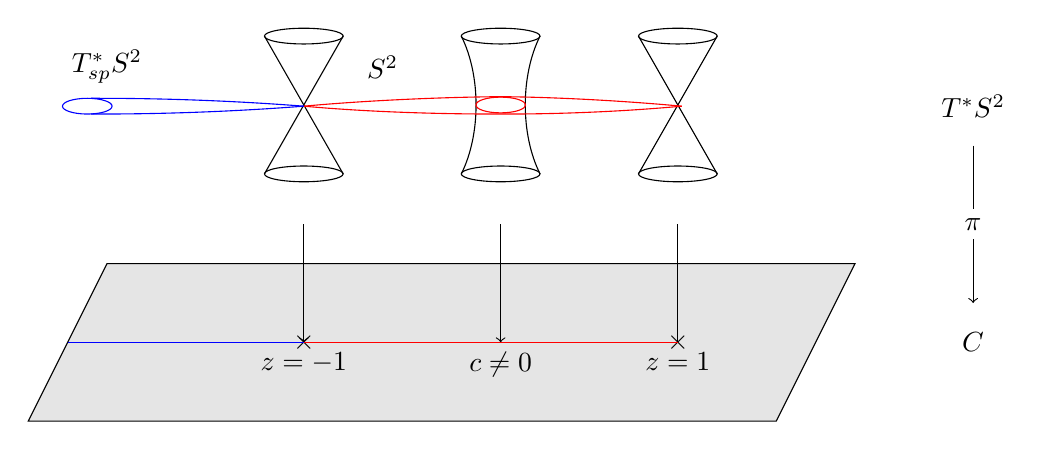
\begin{tikzpicture}

\draw[fill=gray!20] (-2.5,2.5) -- (-3.5,0.5) -- (6,0.5) -- (7,2.5) -- cycle;
\begin{scope}[scale=0.5, shift={(4,3.78)}]
\draw  (-4,7) ellipse (1 and 0.2);
\draw  (-4,3.5) ellipse (1 and 0.2);
\draw (-5,7) -- (-3,3.5) (-5,3.5) -- (-3,7);
\end{scope}
\begin{scope}[scale=0.5, shift={(13.5,3.78)}]
\draw  (-4,7) ellipse (1 and 0.2);
\draw  (-4,3.5) ellipse (1 and 0.2);
\draw (-5,7) -- (-3,3.5) (-5,3.5) -- (-3,7);
\end{scope}
\begin{scope}[scale=0.5,shift={(9,3.78)}]
\draw  (-4,7) ellipse (1 and 0.2);
\draw  (-4,3.5) ellipse (1 and 0.2);

\draw (-5,7) .. controls (-4.5,6) and (-4.5,4.5) .. (-5,3.5);
\draw (-3,7) .. controls (-3.5,6) and (-3.5,4.5) .. (-3,3.5);
\draw[red]  (-4,5.25) ellipse (0.63 and 0.2);
\end{scope}

\draw[->] (2.5,3) -- (2.5,1.5);
\draw[->](0,3) -- (0,1.5);
\node at (0,1.5) {$\times$};
\node[below] at (0,1.5) {$z=-1$};
\node at (4.75,1.5) {$\times$};
\node[below] at (4.75,1.5) {$z=1$};
\node[below] at (2.5,1.5) {$c\neq 0$};
\node at (8.5,1.5) {$\mathbb C$};
\node at (8.5,4.5) {$T^*S^2$};
\draw[->] (8.5,4) -- (8.5,2);
\node[fill=white] at (8.5,3) {$\pi$};


\draw (4.75,3) -- (4.75,1.5);
\draw[red] (0,4.5) .. controls (1.1,4.6) and (2.2,4.62) .. (2.5,4.62) .. controls (2.8,4.62) and (3.7,4.6) .. (4.8,4.5);

\draw[red,yscale=-1] (0,-4.5) .. controls (1.1,-4.4) and (2.2,-4.4) .. (2.5,-4.4) .. controls (2.8,-4.4) and (3.7,-4.4) .. (4.8,-4.5);
\draw[red] (0,1.5) -- (4.75,1.5);
\node at (1,5) {$S^2$};
\draw[blue] (0,1.5) -- (-3,1.5);

\draw[blue, scale=.5]  (-5.5,9) ellipse (0.63 and 0.2);

\draw[blue] (0,4.5) .. controls (-1.3,4.6) and (-2.3,4.6) .. (-2.7,4.6);
\draw[blue] (0,4.5) .. controls (-1.3,4.4) and (-2.3,4.4) .. (-2.7,4.4);
\node at (-2.5,5) {$T^*_{sp}S^2$};
    \label{fig:vanishingpathonsphere}

\end{tikzpicture}